%%%%%%%%%%%%%%%%%%%%%%%%%%%%%%%%%%%%%%%%%
% Beamer Presentation
% LaTeX Template
% Version 1.0 (10/11/12)
%
% This template has been downloaded from:
% http://www.LaTeXTemplates.com
%
% License:
% CC BY-NC-SA 3.0 (http://creativecommons.org/licenses/by-nc-sa/3.0/)
%
%%%%%%%%%%%%%%%%%%%%%%%%%%%%%%%%%%%%%%%%%

%----------------------------------------------------------------------------------------
%	PACKAGES AND THEMES
%----------------------------------------------------------------------------------------

%\documentclass[UTF8,aspectratio=169,14pt]{ctexbeamer}
\documentclass[UTF8,aspectratio=169]{ctexbeamer}
\usepackage{hyperref}
\hypersetup{
	colorlinks=true,
	linkcolor=red,
	anchorcolor=blue,
	citecolor=green
}

\mode<presentation> {
	
	% The Beamer class comes with a number of default slide themes
	% which change the colors and layouts of slides. Below this is a list
	% of all the themes, uncomment each in turn to see what they look like.
	
	%\usetheme{default}
	%\usetheme{AnnArbor}
	%\usetheme{Antibes}
	%\usetheme{Bergen}
	%\usetheme{Berkeley}
	%\usetheme{Berlin}
	%\usetheme{Boadilla}
	%\usetheme{CambridgeUS}
	%\usetheme{Copenhagen}
	%\usetheme{Darmstadt}
	%\usetheme{Dresden}
	%\usetheme{Frankfurt}
	%\usetheme{Goettingen}
	%\usetheme{Hannover}
	%\usetheme{Ilmenau}
	%\usetheme{JuanLesPins}
	%\usetheme{Luebeck}
	\usetheme{Madrid}
	%\usetheme{Malmoe}
	%\usetheme{Marburg}
	%\usetheme{Montpellier}
	%\usetheme{PaloAlto}
	%\usetheme{Pittsburgh}
	%\usetheme{Rochester}
	%\usetheme{Singapore}
	%\usetheme{Szeged}
	%\usetheme{Warsaw}
	
	% As well as themes, the Beamer class has a number of color themes
	% for any slide theme. Uncomment each of these in turn to see how it
	% changes the colors of your current slide theme.
	
	%\usecolortheme{albatross}
	%\usecolortheme{beaver}
	%\usecolortheme{beetle}
	%\usecolortheme{crane}
	%\usecolortheme{dolphin}
	%\usecolortheme{dove}
	%\usecolortheme{fly}
	%\usecolortheme{lily}
	%\usecolortheme{orchid}
	%\usecolortheme{rose}
	%\usecolortheme{seagull}
	%\usecolortheme{seahorse}
	%\usecolortheme{whale}
	%\usecolortheme{wolverine}
	
	%\setbeamertemplate{footline} % To remove the footer line in all slides uncomment this line
	%\setbeamertemplate{footline}[page number] % To replace the footer line in all slides with a simple slide count uncomment this line
	
	%\setbeamertemplate{navigation symbols}{} % To remove the navigation symbols from the bottom of all slides uncomment this line
}

\usepackage{graphicx} % Allows including images
\graphicspath{{./figs/}}
\usepackage{booktabs} % Allows the use of \toprule, \midrule and \bottomrule in tables
\usepackage{longtable}
\usepackage{listings}
\usepackage{xcolor}
\lstset{numbers=left, %设置行号位置
	numberstyle=\tiny, %设置行号大小
	keywordstyle=\color{blue}, %设置关键字颜色
	commentstyle=\color[cmyk]{1,0,1,0}, %设置注释颜色
	frame=single, %设置边框格式
	escapeinside=``, %逃逸字符(1左面的键),用于显示中文
	%breaklines, %自动折行
	extendedchars=false, %解决代码跨页时,章节标题,页眉等汉字不显示的问题
	xleftmargin=2em,xrightmargin=2em, aboveskip=1em, %设置边距
	tabsize=4, %设置tab空格数
	showspaces=false %不显示空格
}
% Fonts
% \usepackage{libertine}
% \setmonofont{Courier}
\setCJKsansfont[ItalicFont=Noto Serif CJK SC Black, BoldFont=Noto Sans CJK SC Black]{Noto Sans CJK SC}
\setmainfont[Ligatures={Common,TeX}]{Linux  Libertine O}
\setmonofont[SmallCapsFont={Latin Modern Mono Caps}]{Latin Modern Mono Light}
\setsansfont{Linux Biolinum O}

\logo{
\includegraphics[width=0.55cm,height=0.55cm]{../../thcs-logo.png}}

%----------------------------------------------------------------------------------------
%	TITLE PAGE
%----------------------------------------------------------------------------------------

\title[第4讲]{第4讲 :Optimization of Virtual Machine Monitor} % The short title appears at the bottom of every slide, the full title is only on the title page
\subtitle{第二节:My VM is Lighter (and Safer) than your Container}
\author{陈渝} % Your name
\institute[清华大学] % Your institution as it will appear on the bottom of every slide, may be shorthand to save space
{
	清华大学计算机系 \\ % Your institution for the title page
	\medskip
	\textit{yuchen@tsinghua.edu.cn} % Your email address
}
\date{\today} % Date, can be changed to a custom date


\begin{document}

\begin{frame}
\titlepage % Print the title page as the first slide
\end{frame}

%\begin{frame}
%\frametitle{提纲} % Table of contents slide, comment this block out to remove it
%\tableofcontents % Throughout your presentation, if you choose to use \section{} and \subsection{} commands, these will automatically be printed on this slide as an overview of your presentation
%\end{frame}
%
%%----------------------------------------------------------------------------------------
%%	PRESENTATION SLIDES
%%----------------------------------------------------------------------------------------
%
%%------------------------------------------------
%\section{第一节:课程概述} % Sections can be created in order to organize your presentation into discrete blocks, all sections and subsections are automatically printed in the table of contents as an overview of the talk
%%------------------------------------------------


%-------------------------------------------------
\begin{frame}[plain]
	\frametitle{Problems of VMM}
	
	
	
	\begin{columns}
		
		\begin{column}{.4\textwidth}
			
			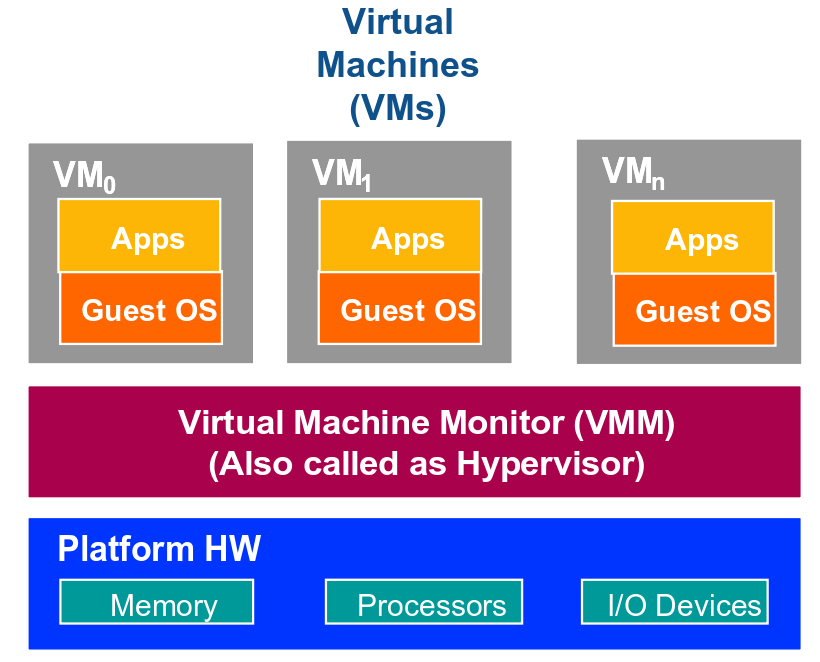
\includegraphics[width=1.\textwidth]{vmm-overview}
			
		\end{column}
		
		\begin{column}{.6\textwidth}
			
			\LARGE
			VMM is \textbf{\underline{SLOWER}} than Container.	
			
			
			
			
			
			
		\end{column}
		
		
	\end{columns}
	
	
\end{frame}


%-------------------------------------------------
\begin{frame}[plain]
	\frametitle{Problems of VMM}
	
	
	
	\begin{columns}
		
		\begin{column}{.5\textwidth}
			
			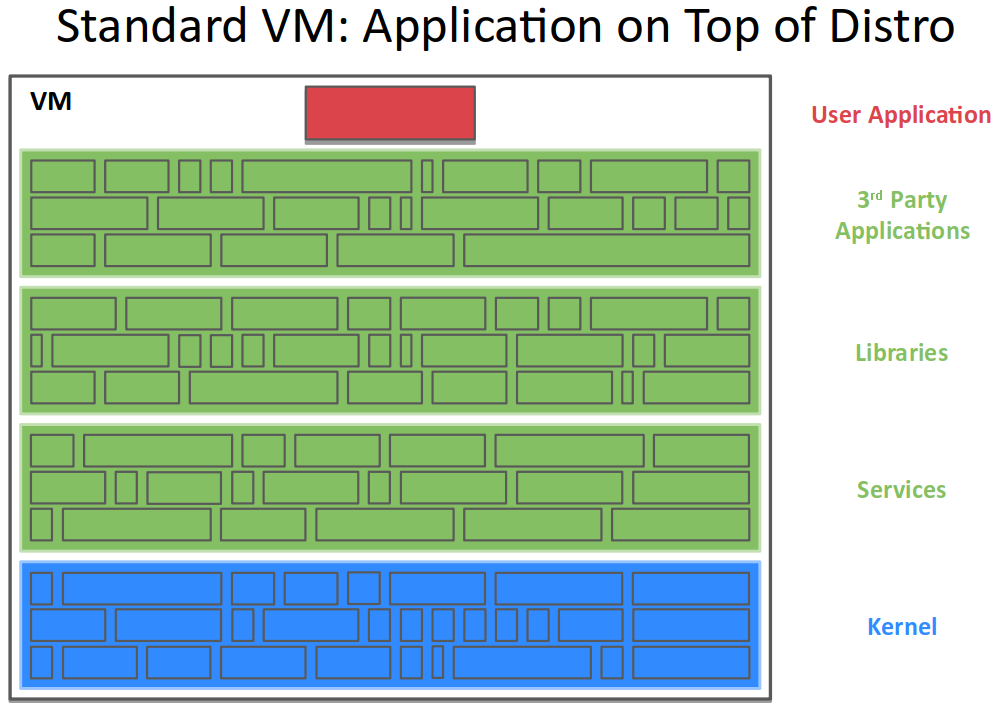
\includegraphics[width=1.\textwidth]{standard-vm}
			
		\end{column}
		
		\begin{column}{.5\textwidth}
			
			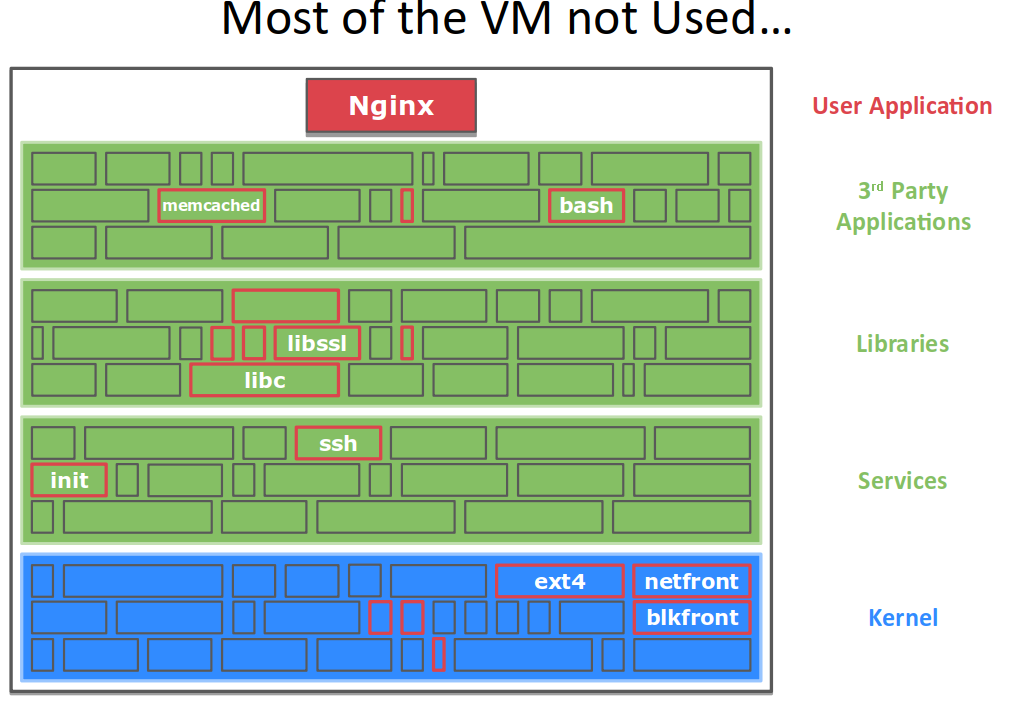
\includegraphics[width=1.\textwidth]{most-vm}
			
			
			
			
			
			
		\end{column}
		
		
	\end{columns}
	
	
\end{frame}

%-------------------------------------------------
\begin{frame}[plain]
	\frametitle{Contributions of lightvm}
	
	
	
	\begin{columns}
		
		\begin{column}{.4\textwidth}
			
			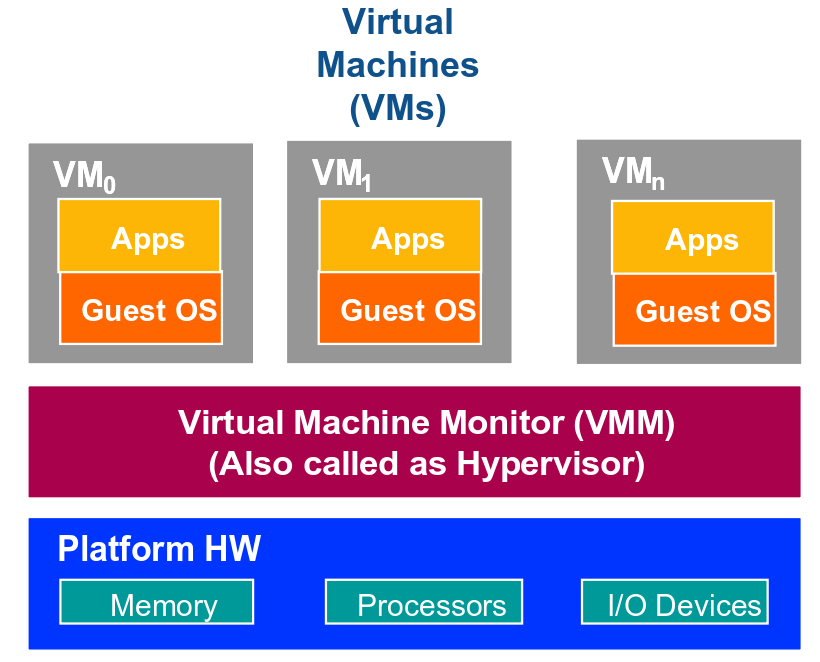
\includegraphics[width=1.\textwidth]{vmm-overview}
			
		\end{column}
		
		\begin{column}{.6\textwidth}
			
			Contributions	
			\begin{itemize}
				\item An analysis of the performance bottlenecks prevent-
				ing traditional virtualization systems from achieving
				container-like dynamics 
				\item An overhaul of Xen’s architecture, completely remov-
				ing its back-end registry 
				\item A revamp of Xen’s toolstack
				\item The development of Tinyx, an automated system for
				building minimalistic Linux-based VMs
				\item A prototypical implementation along with an exten-
				sive performance evaluation 
			\end{itemize}	

%分析了为实现类容器的Dynamics,传统虚拟系统的性能瓶颈在何处。
%重新大改了Xen体系结构,从而显著提高VM的启动和迁移时间。
%修改了Xen的toolstack,包括一些优化和split toolstack的引进。
%split toolstack将可以周期、离线运行的功能与发出命令(例如创建VM)时必须执行的功能分开。
%开发了Tinyx,用于构建基于Linux的最小化VM的自动化系统,同时为Xen开发了许多基于Unikernel内核的应用。
%一个原型实现和性能评估表明,LightVM能够在短至2.3ms的时间内启动(unikernel)VM

		\end{column}
		
		
	\end{columns}
	
	
\end{frame}



%-------------------------------------------------
\begin{frame}[plain]
	\frametitle{Overview of XEN}
	
	
	
	\begin{columns}
		
		\begin{column}{.5\textwidth}
			The Xen architecture including toolstack, the
			XenStore, software switch and split drivers between
			the driver domain (Dom0) and the guests (DomUs).
			
			\centering
			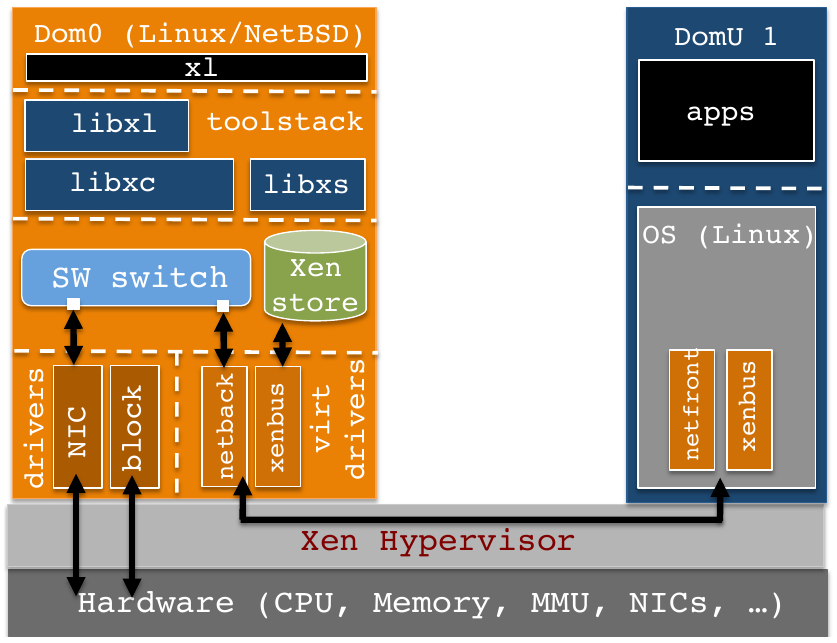
\includegraphics[width=.9\textwidth]{xen-arch2}
			
		\end{column}
		
		\begin{column}{.5\textwidth}
			\centering
			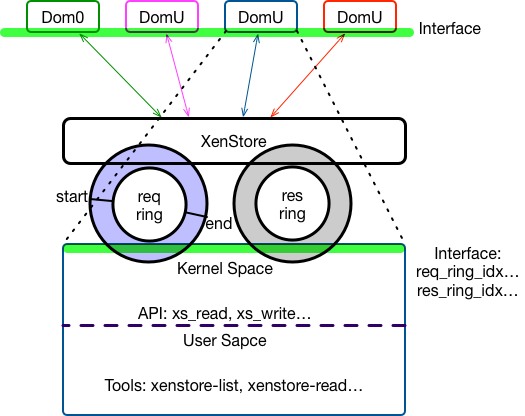
\includegraphics[width=.8\textwidth]{xenstore}
			
%			Contributions	
%			\begin{itemize}
%				\item An analysis of the performance bottlenecks prevent-
%				ing traditional virtualization systems from achieving
%				container-like dynamics 
%				\item An overhaul of Xen’s architecture, completely remov-
%				ing its back-end registry 
%				\item A revamp of Xen’s toolstack
%				\item The development of Tinyx, an automated system for
%				building minimalistic Linux-based VMs
%				\item A prototypical implementation along with an exten-
%				sive performance evaluation 
%			\end{itemize}	
			
		\end{column}
		
		
	\end{columns}
	
	
\end{frame}




%-------------------------------------------------
\begin{frame}[plain]
	\frametitle{Some observations on XEN }
	
	
	
	\begin{columns}
		
		\begin{column}{.3\textwidth}
			The Xen architecture including toolstack, the
			XenStore, software switch and split drivers between
			the driver domain (Dom0) and the guests (DomUs).
			
			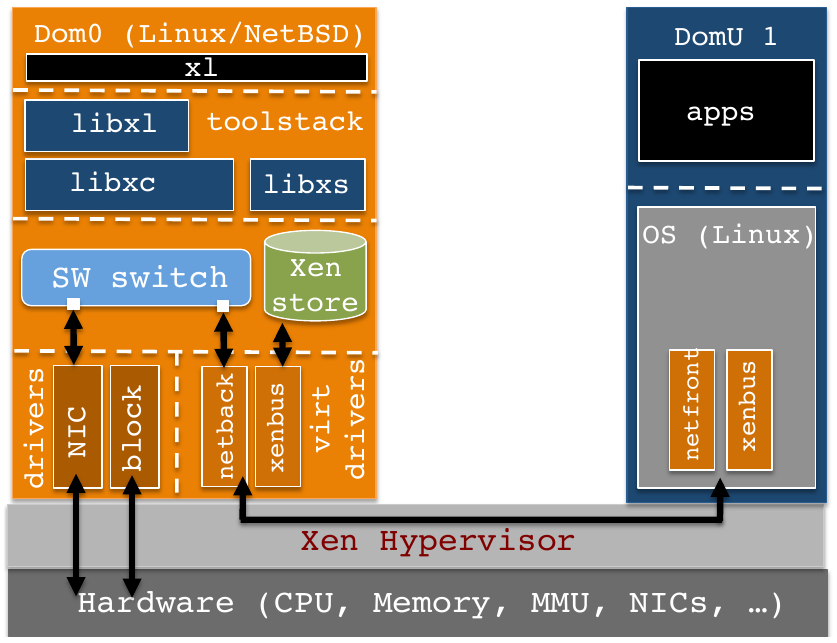
\includegraphics[width=1.\textwidth]{xen-arch2}
			
		\end{column}
		
		\begin{column}{.7\textwidth}
			
			\small The size of the guest virtual machines
			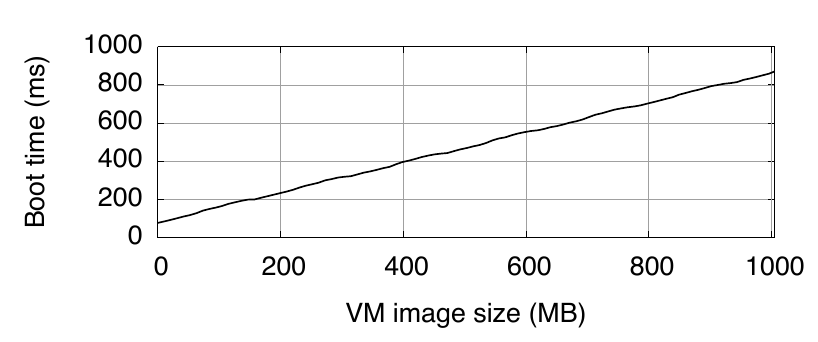
\includegraphics[width=1.\textwidth]{vmm-boot-time}
%			\small sequentially start 1000 virtual machines 
%			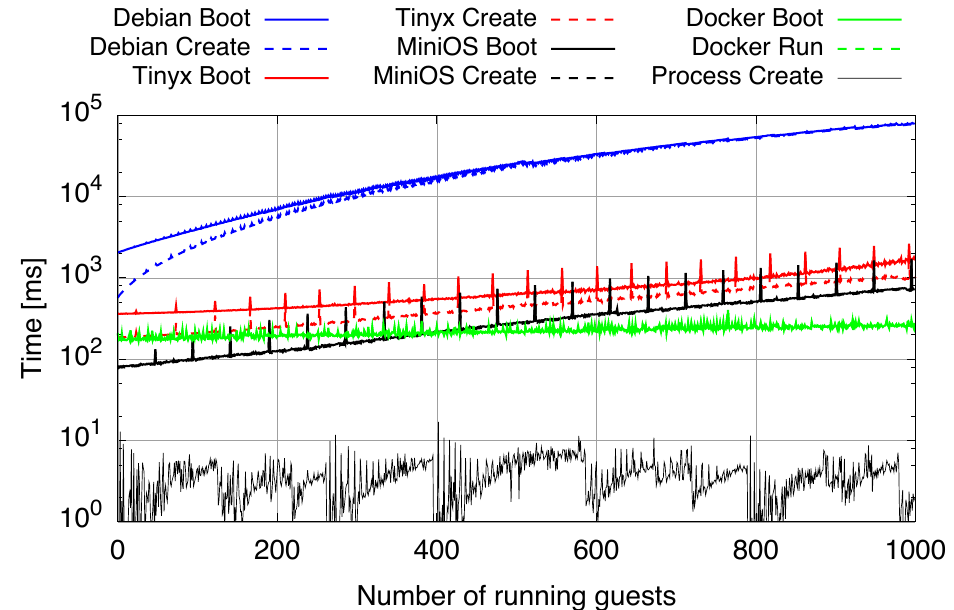
\includegraphics[width=.7\textwidth]{bench-vm-create}
		\end{column}
		
		
	\end{columns}
	
	
\end{frame}


%-------------------------------------------------
\begin{frame}[plain]
	\frametitle{LIGHTWEIGHT VMs }
	
	
	
	\begin{columns}
		
		\begin{column}{.3\textwidth}
		
			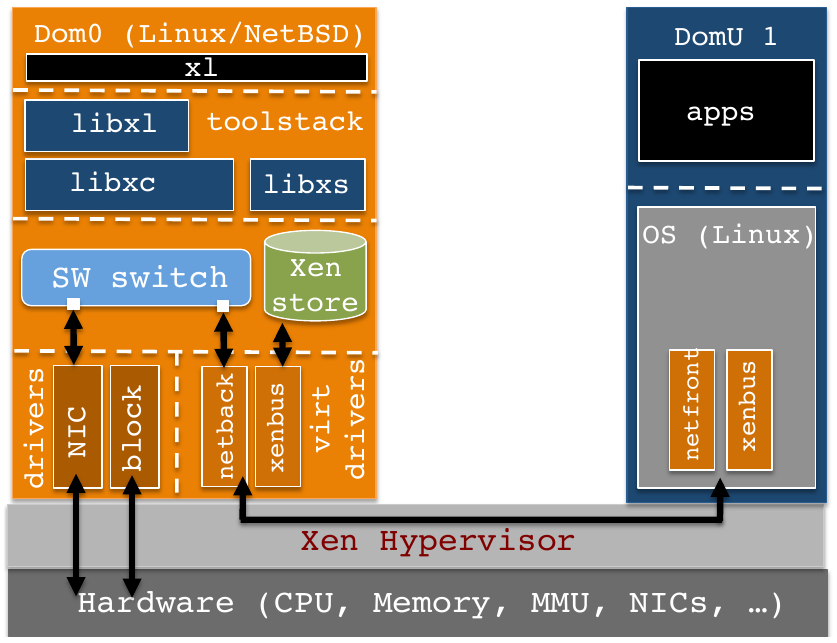
\includegraphics[width=1.\textwidth]{xen-arch2}
			
		\end{column}
		
		\begin{column}{.7\textwidth}
			
\begin{itemize}			
	\item \textbf{Unikernels:} 
	linking existing applications that rely
	on the Linux syscall API to Mini-OS is fairly cumbersome and
	requires a lot of expert time.
	
	\item \textbf{Tinyx: }is an automated build system that creates minimalistic
	Linux VM images targeted at running a single application  
\end{itemize}

		\end{column}
		
		
	\end{columns}
	
	
\end{frame}

%-------------------------------------------------
\begin{frame}[plain]
	\frametitle{LIGHTWEIGHT VMs }
	
	
	
	\begin{columns}
		
		\begin{column}{.3\textwidth}
			
			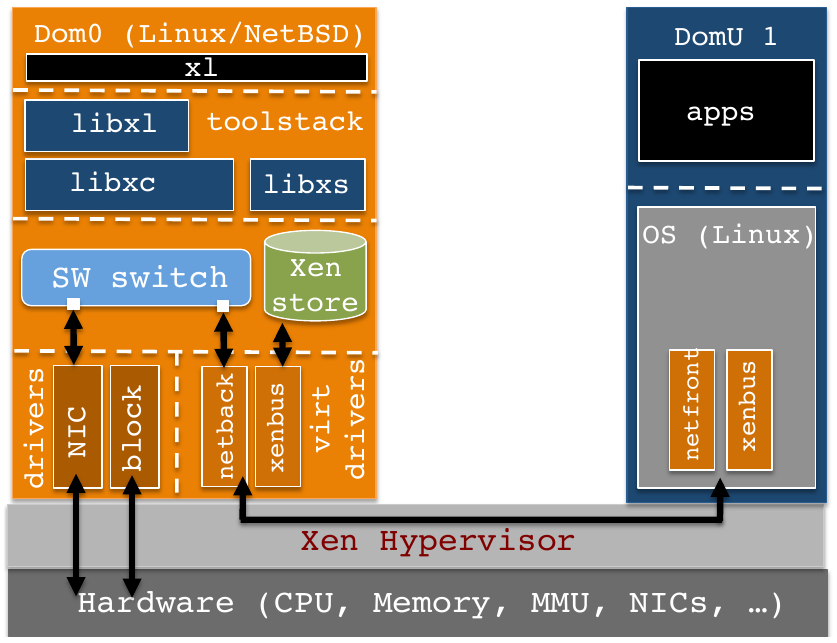
\includegraphics[width=1.\textwidth]{xen-arch2}
			
		\end{column}
		
		\begin{column}{.7\textwidth}
			\textbf{Tinyx: }
			\begin{itemize}			
				
				\item Inputs: an application to build the image for and the platform the image	will be running on.
				\item Includes: the application, its dependencies,	and BusyBox 
				\item Methods: objdump for libs, pkg manager for packages, tinyconfig for Linux kernel.
				\item Results:  Tinyx create kernel images that are half the size of typical		Debian kernels and minimal runtime memory usage
				\item (1.6MB for Tinyx vs. 8MB for the Debian)
				
				
			\end{itemize}
			
		\end{column}
		
		
	\end{columns}
	
	
\end{frame}

%-------------------------------------------------
\begin{frame}[plain]
	\frametitle{Some observations on XEN }
	
	
	
	\begin{columns}
		
		\begin{column}{.4\textwidth}

\begin{itemize}			
\item The Debian VM is 1.1GB; 
it takes Xen around 500ms
to create the VM, and
it takes the VM 1.5 seconds to boot. 

\item The Tinyx VM (9.5MB) is created in 360ms and  180ms to boot.
The unikernel (480KB) is created in 80ms, and
3ms to boot.

\item  Creating VMs, the creation time
increases noticeably (note the logarithmic scale): it takes 42s, 10s and 700ms to create the thousandth Debian, Tinyx, and unikernel guest,

\end{itemize}
			
		\end{column}
		
		\begin{column}{.6\textwidth}
			
%			\small The size of the guest virtual machines
%			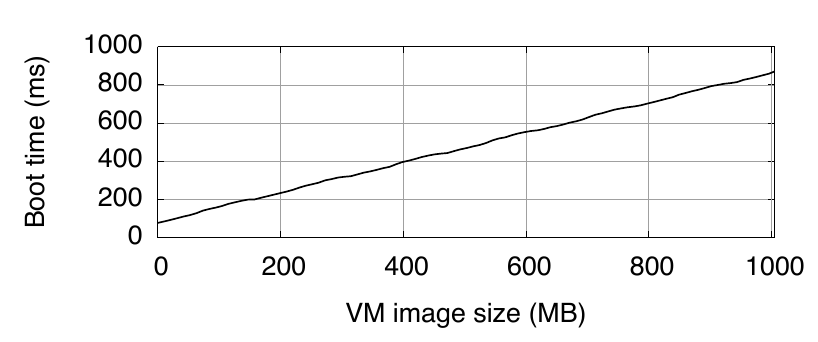
\includegraphics[width=.8\textwidth]{vmm-boot-time}
			\small sequentially start 1000 virtual machines 
			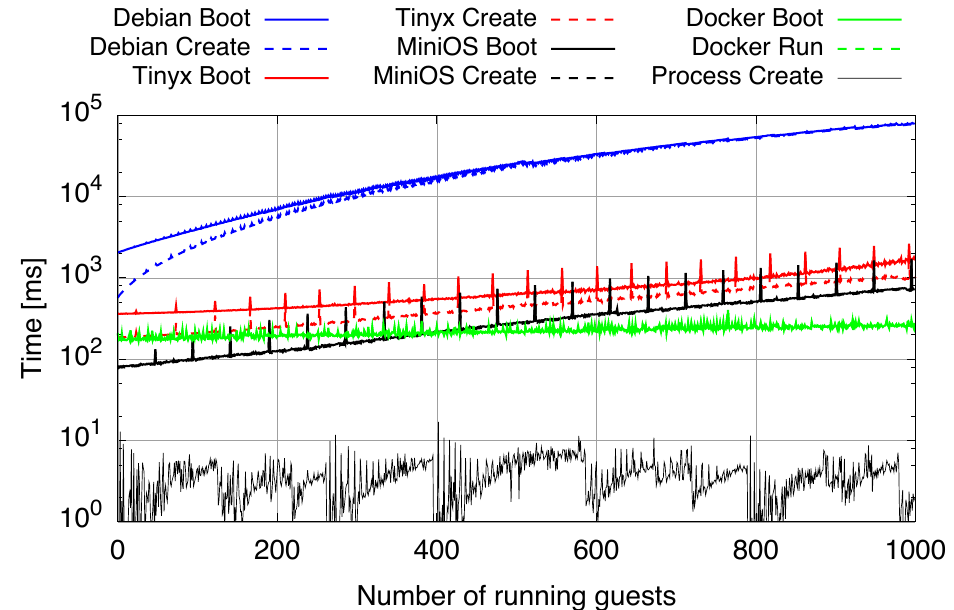
\includegraphics[width=1.\textwidth]{bench-vm-create}
		\end{column}
		
		
	\end{columns}
	
	
\end{frame}



%-------------------------------------------------
\begin{frame}[plain]
	\frametitle{Some observations on XEN }
	
	
	
	\begin{columns}
		
		\begin{column}{.4\textwidth}
			 VM creation overheads
			\begin{itemize}			
				\item Parsing the configuration file that describes the VM
				\item  Interacting with the hypervisor for memory
				\item  Reading/Writing information in XenStore
				\item  Creating and configuration the virtual devices
				\item Parsing \& loading the kernel image 
				\item Other work on toolstack
				
			\end{itemize}
			
		\end{column}
		
		\begin{column}{.6\textwidth}
			
			%			\small The size of the guest virtual machines
			%			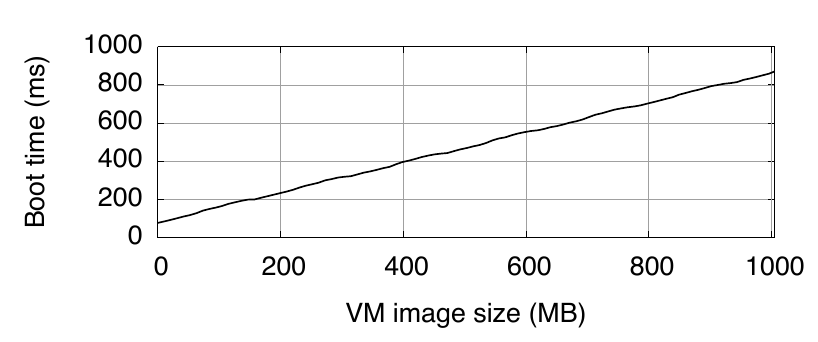
\includegraphics[width=.8\textwidth]{vmm-boot-time}
			\small Breakdown of the VM creation overheads 
			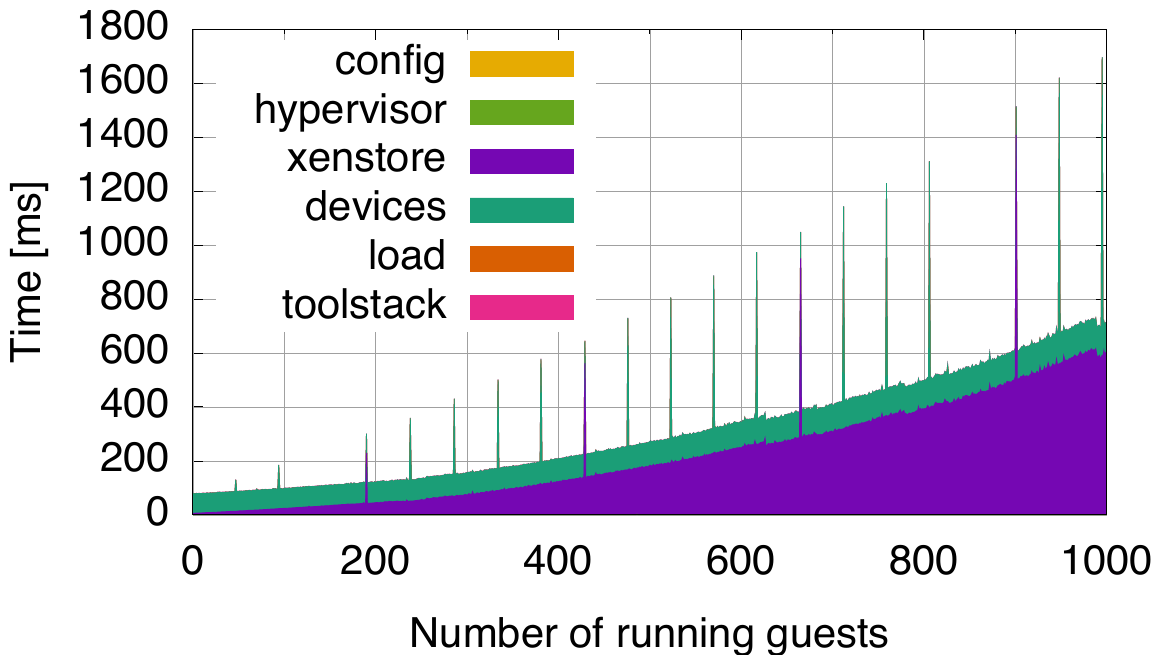
\includegraphics[width=1.\textwidth]{breakdown-vm-create}
		\end{column}
		
		
	\end{columns}
	
	
\end{frame}



%-------------------------------------------------
\begin{frame}[plain]
	\frametitle{LightVM }
	
	
	
	\begin{columns}
		
		\begin{column}{.5\textwidth}
			\centering XEN
			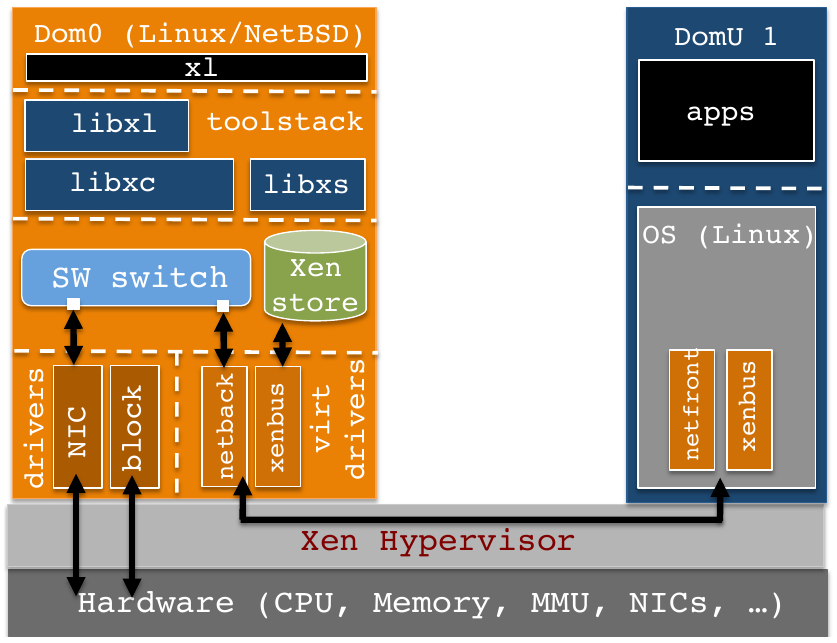
\includegraphics[width=1.\textwidth]{xen-arch2}
			
		\end{column}
		
		\begin{column}{.5\textwidth}
			LightVM with Noxs and the Chaos
			Toolstack
			
			\centering
			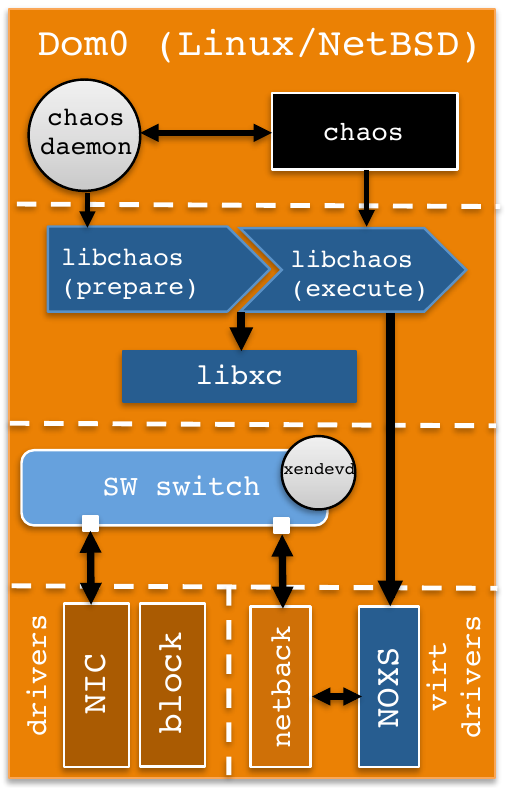
\includegraphics[width=.6\textwidth]{lightvm}

			
		\end{column}
		
		
	\end{columns}
	
	
\end{frame}
%-------------------------------------------------


%-------------------------------------------------
\begin{frame}[plain]
	\frametitle{LightVM -- noxs}
	
	
	
	\begin{columns}
		
		\begin{column}{.5\textwidth}
		

		\centering
		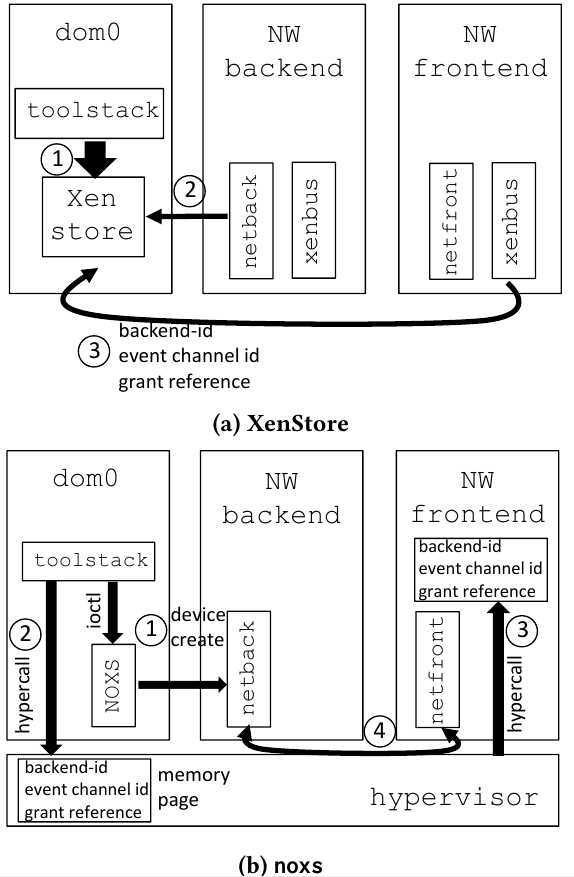
\includegraphics[width=.65\textwidth]{xenstore-noxs}
			
		\end{column}
		
		\begin{column}{.5\textwidth}

		\begin{itemize}			
			\item fundamental problem with the XenStore is its
			centralized, filesystem-like API
			\item  noxs relies on shared pages mapped in the guest's address space
			\item create a new,
			special device memory page for each new VM that we use
			to keep track of a VM's information about any devices
			
		\end{itemize}
			
			
		\end{column}
		
		
	\end{columns}
	
	
\end{frame}



%-------------------------------------------------
\begin{frame}[plain]
	\frametitle{LightVM -- noxs }
	
	
	
	\begin{columns}
		
		\begin{column}{.5\textwidth}
			
			
			\centering
			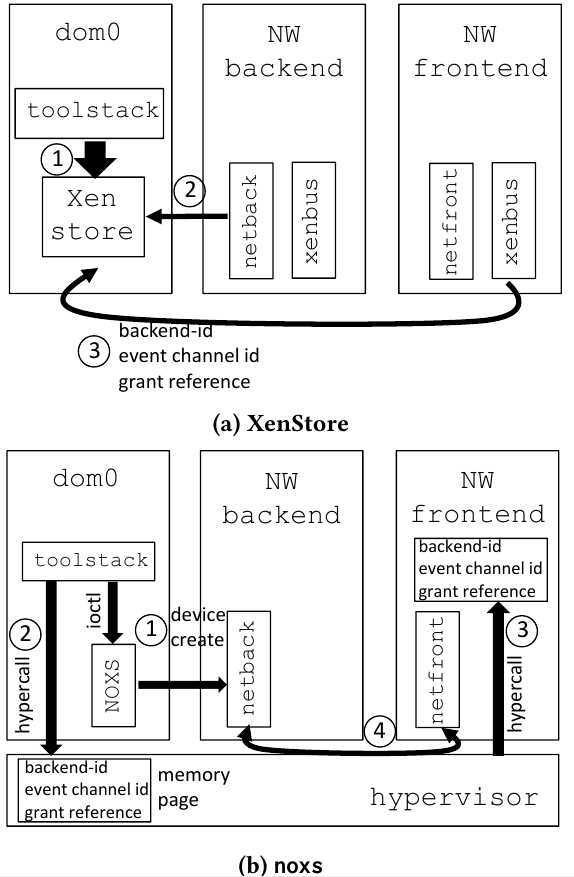
\includegraphics[width=.65\textwidth]{xenstore-noxs}
			
		\end{column}
		
		\begin{column}{.5\textwidth}
			
			\begin{itemize}			
				\item toolstack requests the creation of devices from the back-end
				\item toolstack calls the new hypercall for adding these details to the device page
				\item New VM maps the device page into its address space
				\item front-end inits comm. with back-end
				\item finally front-end and back-end can notify each other
				
				
			\end{itemize}
			
			
		\end{column}
		
		
	\end{columns}
	
	
\end{frame}
%-------------------------------------------------


%-------------------------------------------------
\begin{frame}[plain]
	\frametitle{LightVM -- split toolstack }
	
	
	
	\begin{columns}
		
		\begin{column}{.6\textwidth}
			
			
			\centering
			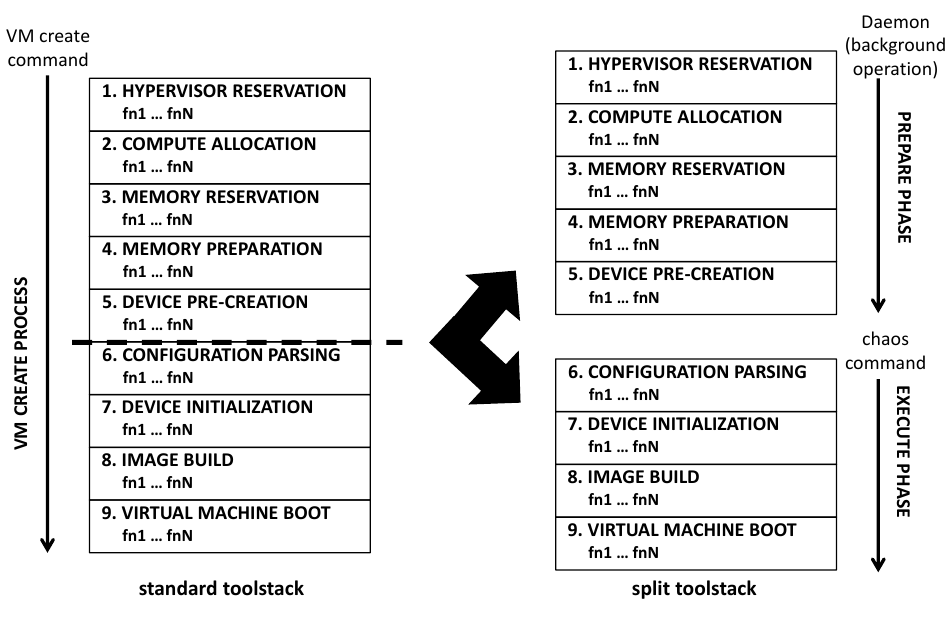
\includegraphics[width=1.\textwidth]{split-toolstack}
			
		\end{column}
		
		\begin{column}{.4\textwidth}
			
			\begin{itemize}			
				\item Toolstack split between functionality belonging to the prepare phase, carried out periodically
				by the chaos daemon,
				\item offload this functionality to the chaos daemon, which generates a number
				of VM shells and places them in a pool. 
				\item and an execute phase, directly
				called by chaos when a command is issued.
				
				
				
			\end{itemize}
			
			
		\end{column}
		
		
	\end{columns}
	
	
\end{frame}



%-------------------------------------------------
\begin{frame}[plain]
	\frametitle{LightVM -- Performance}
	
	
	
	\begin{columns}
		
		\begin{column}{.3\textwidth}
			\centering LightVM
			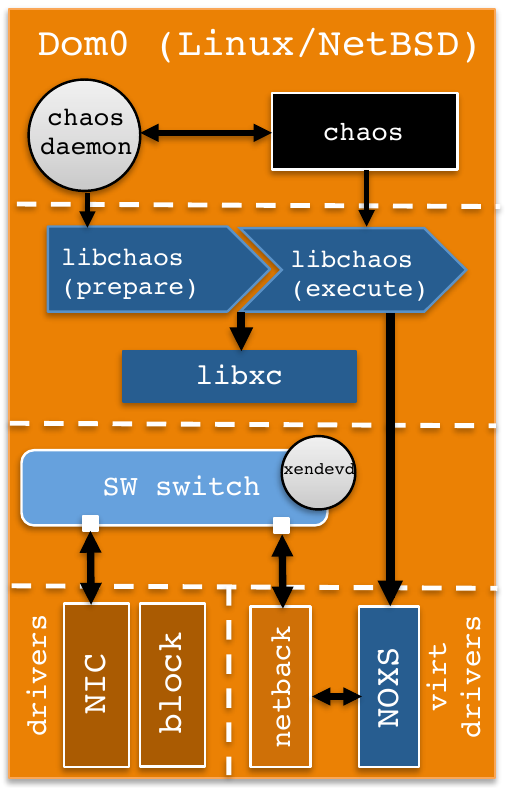
\includegraphics[width=1.\textwidth]{lightvm}
			
		\end{column}
		
		\begin{column}{.7\textwidth}
			LightVM with Noxs and the Chaos
			Toolstack
			
			\centering
			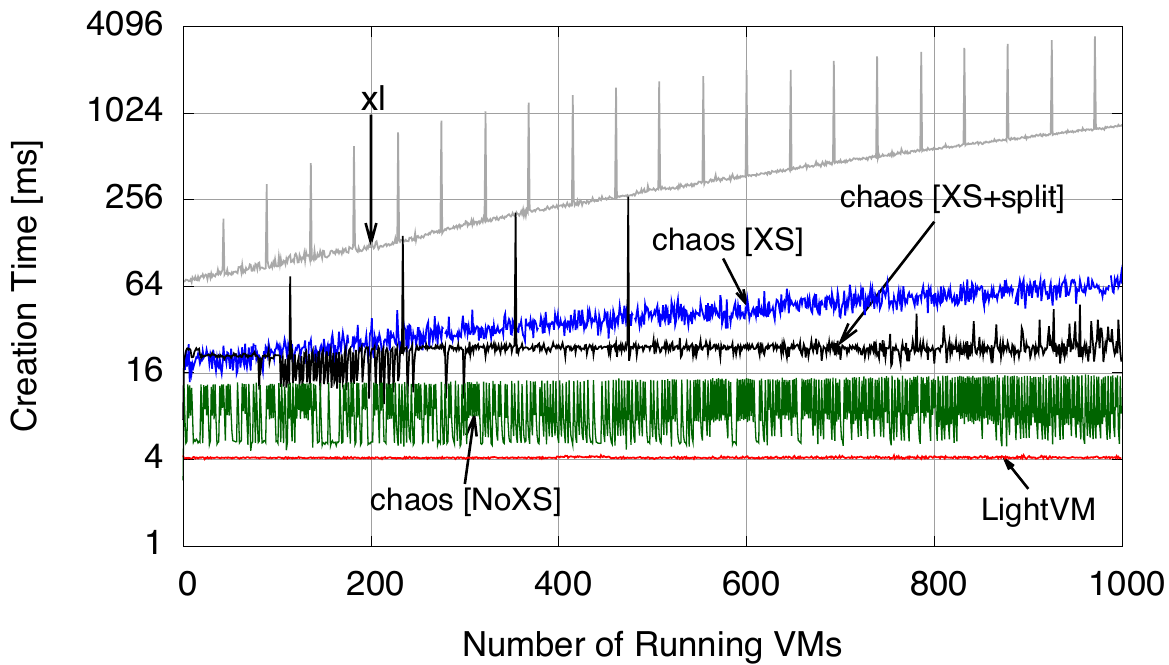
\includegraphics[width=1.\textwidth]{creation-perfs}
			
			
		\end{column}
		
		
	\end{columns}
	
	
\end{frame}


%-------------------------------------------------
\begin{frame}[plain]
	\frametitle{LightVM -- Performance}
	
	
	
	\begin{columns}
		
		\begin{column}{.5\textwidth}
			LightVM boot times on a 64-core machine
			versus Docker containers.
			
			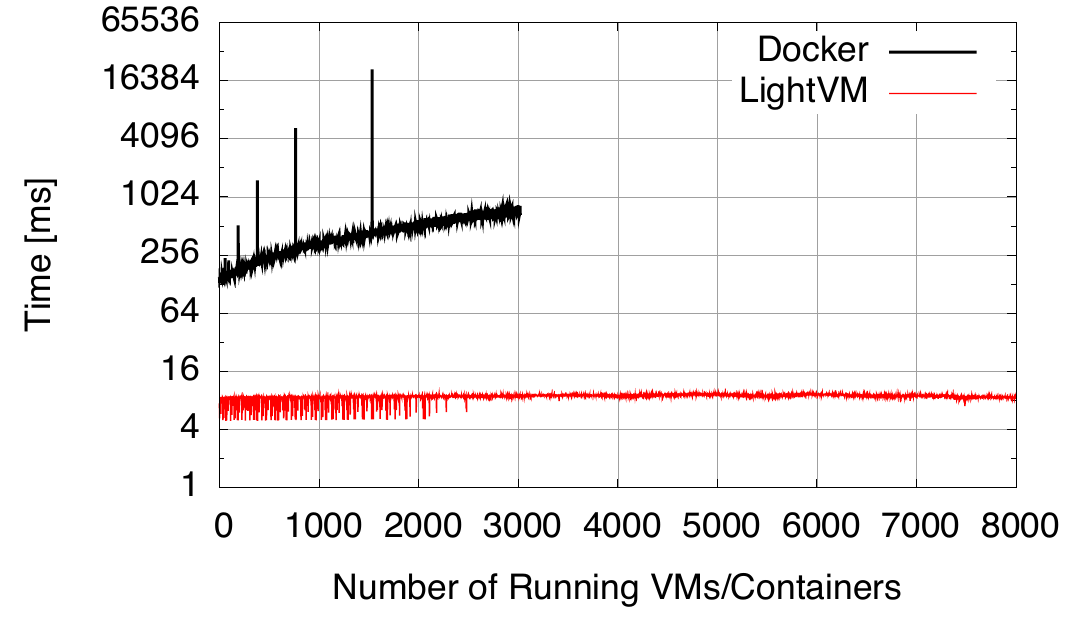
\includegraphics[width=1.\textwidth]{boottime-lvm-cont}
			
		\end{column}			
		
		\begin{column}{.5\textwidth}
			Boot times for unikernel and Tinyx guests
			versus Docker containers
			
			\centering
			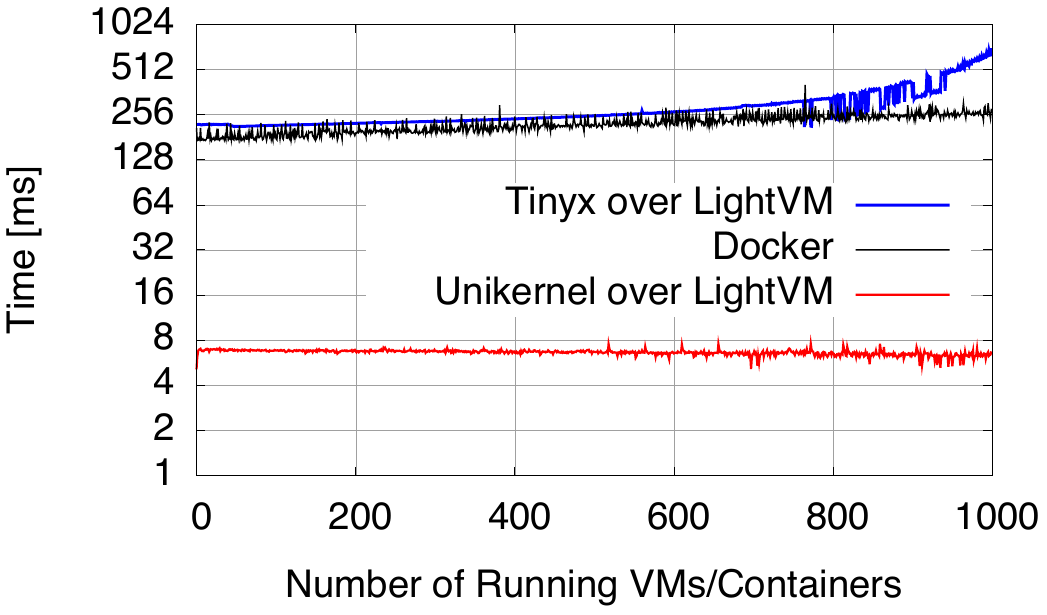
\includegraphics[width=1.\textwidth]{boottime-guest-cont}
			
			
		\end{column}
		
		
	\end{columns}
	
	
\end{frame}


%-------------------------------------------------
\begin{frame}[plain]
	\frametitle{LightVM -- Performance}
	
	
	
	\begin{columns}
		
		\begin{column}{.5\textwidth}
			Scalability of VM memory usage for different VMs, for containers and for processes.
			
			
			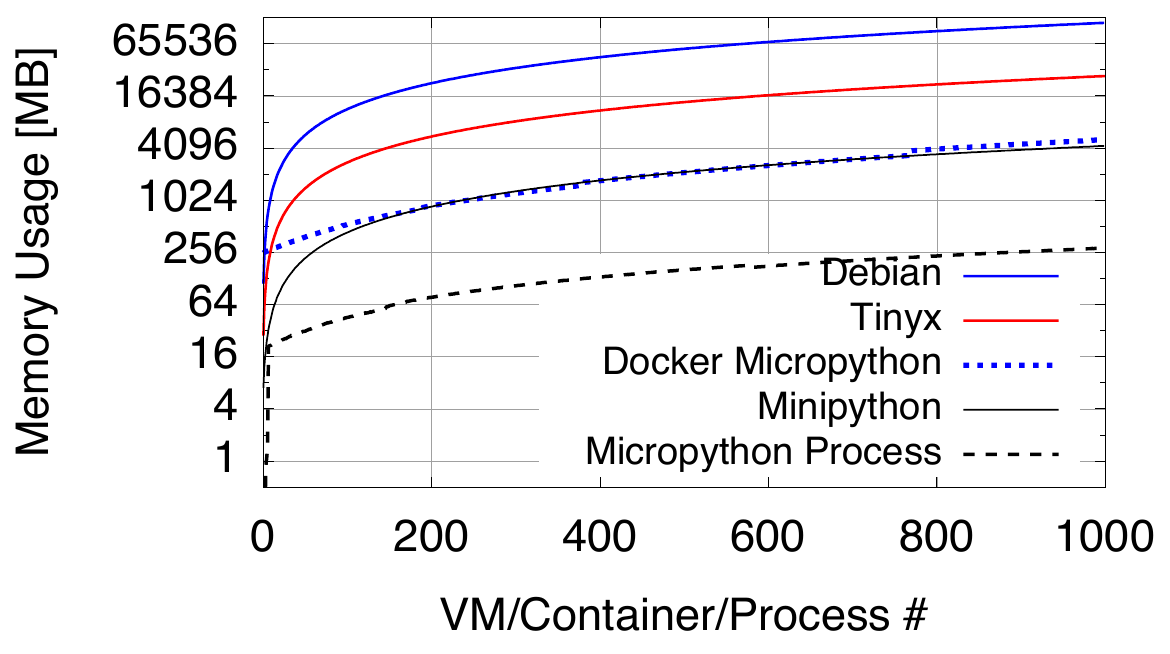
\includegraphics[width=1.\textwidth]{vm-mem-usage}
			
		\end{column}
		
		\begin{column}{.5\textwidth}			

			CPU usage for a unikernel, Tinyx, a Debian
			VM and Docker.
			
			
			\centering
			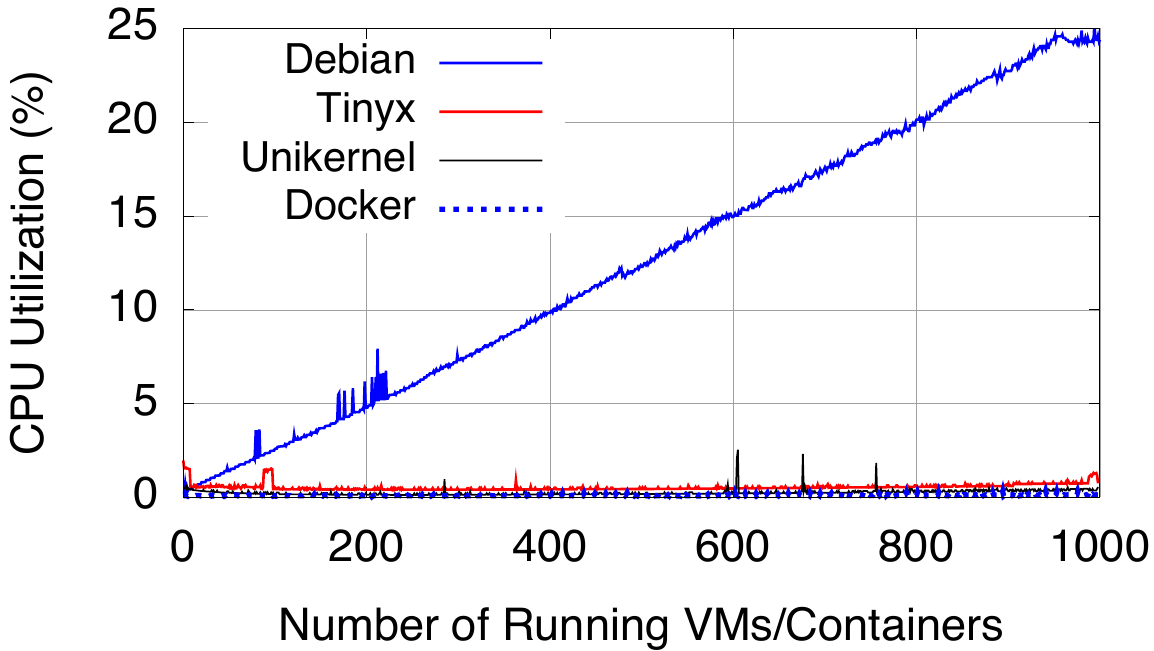
\includegraphics[width=1.\textwidth]{vm-cpu-usage}
			
			
		\end{column}
		
		
	\end{columns}
	
	
\end{frame}
%-------------------------------------------------

%-------------------------------------------------
\begin{frame}[plain]
	\frametitle{LightVM -- Summary}
	
	LightVM
\begin{itemize}			
	\item  A complete redesign of Xen's toolstack optimized for performance.
	\item Can boot a minimalistic VM in as little as 2.3ms, comparable to the fork/exec implementation in Linux (1ms).  
	\item Has almost
	constant creation and boot times regardless of the number
	of running VMs.
	\item  Achieve both good isolation and performance
	on par or better than containers. 
	
	
\end{itemize}	

	
\end{frame}
%-------------------------------------------------
%-------------------------------------------------
\end{document}